\documentclass[10pt,twocolumn]{article}

% ------------------------------------------------------------
% Packages
% ------------------------------------------------------------
\usepackage[margin=0.72in]{geometry}
\usepackage{times}
\usepackage{graphicx}
\usepackage{booktabs}
\usepackage{multirow}
\usepackage{amsmath,amssymb}
\usepackage{array}
\usepackage{xcolor}
\usepackage{enumitem}
\usepackage{caption}
\usepackage{subcaption}
\usepackage{hyperref}
\usepackage{float}
\usepackage{balance}
\usepackage[section]{placeins}
\usepackage{dblfloatfix}

\hypersetup{
    colorlinks=true,
    linkcolor=blue,
    citecolor=blue,
    urlcolor=blue
}

\graphicspath{{figures/}}

% Compact table settings
\setlength{\tabcolsep}{4pt}
\renewcommand{\arraystretch}{1.05}
\setlist[itemize]{leftmargin=*, topsep=2pt, itemsep=1pt}

% ------------------------------------------------------------
% Title
% ------------------------------------------------------------
\title{FastGainRouter: Input-Adaptive Efficient Restoration for Smartphone Images with Dirty Lenses}

\author{
Donggyun Seo \\
Department of AI Software, Soongsil University \\
\texttt{[TODO: your-email@example.com]}
}
\date{}

\begin{document}
\maketitle

% ------------------------------------------------------------
% Abstract
% ------------------------------------------------------------
\begin{abstract}
Smartphone images captured through contaminated lenses suffer from spatially varying degradations such as dust, fingerprints, water droplets, scratches, and mixed lens artifacts.
The SIDL benchmark introduced this realistic dirty-lens restoration problem and evaluated existing restoration models under fixed-model inference.
However, applying the same restoration model to every input may be unnecessary or even suboptimal: some images are already close to the reference, some can be sufficiently restored by a lightweight model, and only a subset benefits from a stronger model.
We study input-adaptive restoration budget selection for SIDL and propose \textbf{FastGainRouter}, a lightweight routing framework that selects one of three branches: \textit{Input}, which bypasses restoration; \textit{Tiny}, a width-4 NAFNet-based lightweight model; and \textit{Base}, a width-8 NAFNet-based stronger model.
Instead of predicting a hard oracle branch label, the router predicts two restoration gains: the expected improvement of Tiny over Input and the additional improvement of Base over Tiny.
On the official SIDL validation set, Tiny improves PSNR over Input by 1.315 dB on average, while Base improves over Tiny by only 0.106 dB on average.
In the balanced setting, FastGainRouter improves PSNR over Always Base by 0.031 dB while reducing component-based latency by 9.1\%.
In the efficient setting, it reduces latency by 18.5\% with only 0.066 dB PSNR loss.
These results suggest that input-adaptive restoration budget selection is a promising direction for efficient dirty-lens image restoration.
\end{abstract}

% ------------------------------------------------------------
% 1. Introduction
% ------------------------------------------------------------
\section{Introduction}

Smartphone cameras are ubiquitous in daily life, but their image quality can be significantly degraded by contaminated lenses.
In real usage, lenses are frequently affected by water droplets, dust, fingerprints, scratches, and combinations of such contaminants.
These degradations differ from standard image restoration problems such as Gaussian denoising, motion deblurring, or synthetic haze removal.
Since the artifact is introduced at the lens surface before image formation, dirty-lens degradation can cause spatially non-uniform blur, light scattering, local occlusion, contrast reduction, and color distortion.

The SIDL benchmark introduced a real-world dataset for restoring smartphone images captured through dirty lenses \cite{sidl2025}.
It provides paired degraded and clean reference images and evaluates representative restoration models such as AirNet, NAFNet, Restormer, FFTformer, DiffUIR, AutoDIR, and MambaIR.
The Easy, Medium, and Hard categories in SIDL are used for evaluation and analysis rather than for dynamic model selection.
Thus, SIDL primarily answers the question: \textit{how well does a fixed restoration model perform on dirty-lens images?}

In this work, we ask a complementary question: \textit{does every dirty-lens image require the same restoration budget?}
Some images are already close to their reference images, and applying a restoration model may introduce unnecessary smoothing or color shifts.
Some images can be sufficiently restored by a small model, while only a subset benefits from a stronger model.
Therefore, fixed-model restoration may be inefficient because it applies the same computational budget to all inputs.

We formulate dirty-lens restoration as an input-adaptive branch selection problem.
Given a degraded input image, our system selects one of three branches: \textbf{Input}, \textbf{Tiny}, or \textbf{Base}.
The Input branch bypasses restoration and returns the degraded image unchanged.
The Tiny branch is a lightweight NAFNet-based model, and the Base branch is a stronger NAFNet-based model.
The goal is not to replace the SIDL benchmark or to claim state-of-the-art restoration quality, but to investigate whether input-adaptive restoration budget selection can provide a better quality-efficiency trade-off.

A naive router could be trained to classify the branch with the highest PSNR.
However, this hard oracle label can be unstable when the PSNR difference between two branches is very small.
For example, if Base is only 0.02 dB better than Tiny, treating Base as the only correct class ignores the computational cost of using the stronger model.
Instead, we propose \textbf{FastGainRouter}, which predicts restoration gains rather than hard branch labels.

Our contributions are summarized as follows:
\begin{itemize}
    \item We analyze Input/Tiny/Base branch behavior on SIDL and show that all three branches are optimal for a non-trivial portion of validation samples.
    \item We propose FastGainRouter, a lightweight gain-based routing policy that predicts restoration gains from simple input image statistics.
    \item We demonstrate that FastGainRouter improves the quality-latency trade-off over fixed baselines. In the balanced setting, it improves PSNR over Always Base while reducing component-based latency; in the efficient setting, it achieves larger latency reduction with a small PSNR loss.
\end{itemize}

% ------------------------------------------------------------
% 2. Related Work
% ------------------------------------------------------------
\section{Related Work}

\paragraph{Dirty-lens image restoration.}
Image restoration has traditionally focused on degradations such as denoising, deblurring, super-resolution, deraining, and dehazing.
Dirty-lens degradation is different because the artifact is caused by physical contaminants in front of the camera lens.
SIDL addresses this underexplored problem by collecting paired smartphone images with realistic lens contaminants and clean references \cite{sidl2025}.
Our work builds on SIDL but studies a different question: whether the restoration budget should be selected adaptively for each input rather than applying one fixed model to all images.

\paragraph{Deep image restoration.}
Recent restoration models include CNN-based, transformer-based, and hybrid architectures.
MPRNet uses a multi-stage progressive architecture for image restoration \cite{mprnet2021}.
Restormer introduces an efficient transformer design for high-resolution restoration \cite{restormer2022}.
NAFNet proposes a simple activation-free baseline that achieves strong restoration performance with efficient architecture design \cite{nafnet2022}.
We use NAFNet variants to construct controlled Tiny and Base branches, since our goal is to analyze adaptive budget selection rather than to design a new restoration backbone.

\paragraph{Dynamic inference and adaptive computation.}
Dynamic inference methods allocate computation depending on input difficulty.
BranchyNet introduces early exits to reduce computation for easy samples \cite{branchynet2016}.
SkipNet learns to skip layers dynamically \cite{skipnet2018}.
Slimmable Neural Networks allow inference at different network widths \cite{slimmable2019}, and Once-for-All trains a super-network from which specialized subnetworks can be selected for deployment constraints \cite{onceforall2020}.
Our work shares the motivation that not all inputs require the same computation, but differs in that we route images among restoration branches and use predicted restoration gain as the routing signal.

% ------------------------------------------------------------
% 3. Problem Setting and Dataset
% ------------------------------------------------------------
\section{Problem Setting and Dataset}

\subsection{Input-Adaptive Restoration}

Given a degraded dirty-lens image $x$, a standard restoration pipeline applies a fixed restoration model $f$:
\begin{equation}
    \hat{y} = f(x).
\end{equation}
In contrast, we define a set of candidate branches:
\begin{equation}
    \mathcal{A} = \{\text{Input}, \text{Tiny}, \text{Base}\}.
\end{equation}
The system selects a branch $a(x) \in \mathcal{A}$ for each input and produces:
\begin{equation}
    \hat{y} = f_{a(x)}(x).
\end{equation}
The Input branch is the identity function:
\begin{equation}
    f_{\text{Input}}(x)=x.
\end{equation}

\subsection{Dataset Splits}

We use the SIDL dataset.
The official validation set is kept as the final held-out evaluation set.
The official training split is internally divided at the case level into \textit{train\_inner} and \textit{es\_val\_inner}.
The train\_inner split is used for restoration model training and router gain target generation.
The es\_val\_inner split is used for early stopping, best checkpoint selection, and router threshold tuning.
The official validation set is used only for final evaluation.
Case-level splitting is important because SIDL images are patch-based; multiple patches may originate from the same scene case.

\begin{table}[!t]
\centering
\caption{Split usage in the final experimental protocol.}
\label{tab:split}
\resizebox{\columnwidth}{!}{
\begin{tabular}{llrl}
\toprule
Split & Source & Samples & Usage \\
\midrule
train\_inner & official train & 51,264 & model training, router target generation \\
es\_val\_inner & official train & 5,616 & early stopping, threshold tuning \\
official val & official val & 5,520 & final evaluation only \\
\bottomrule
\end{tabular}
}
\end{table}

\subsection{Evaluation Metrics}

We report PSNR, SSIM, and LPIPS.
PSNR and SSIM measure full-reference fidelity, while LPIPS provides a perceptual similarity measure.
For efficiency, we report a measured component-based latency estimate, which includes fast feature extraction, batch router prediction, and selected branch inference.
We also report pure forward latency for candidate branch analysis.

% ------------------------------------------------------------
% 4. Method
% ------------------------------------------------------------
\section{Method}

\subsection{Overview}

Our method consists of three branches and a lightweight gain router.
Given an input image, we first compute fast image statistics.
FastGainRouter predicts two restoration gains and selects Input, Tiny, or Base using a threshold-based decision rule.
Figure~\ref{fig:overview} illustrates the overall pipeline.

\begin{figure}[!t]
    \centering
    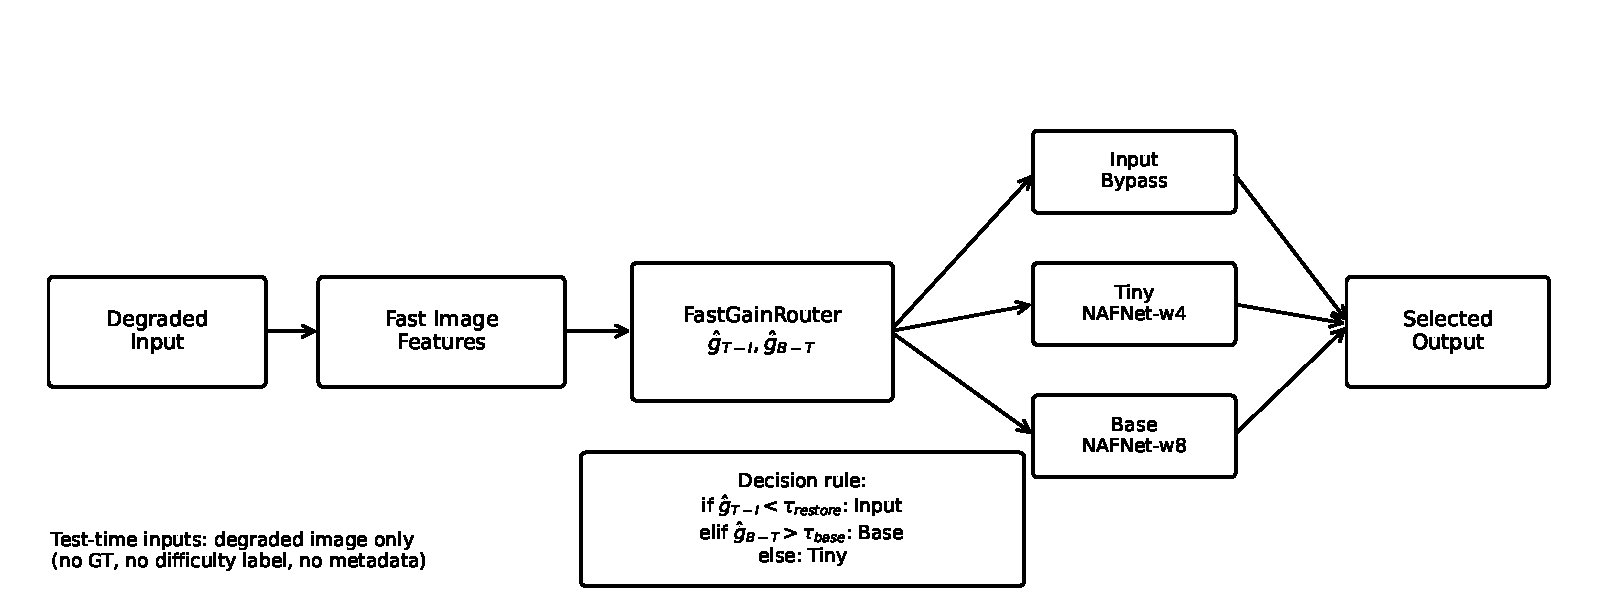
\includegraphics[width=\columnwidth]{method_overview_v1.pdf}
    \caption{
    Overview of FastGainRouter.
    Given a degraded input image, the system extracts lightweight image statistics,
    predicts restoration gains, and routes the sample to Input, Tiny, or Base.
    }
    \label{fig:overview}
\end{figure}

\subsection{Branch Design}

\paragraph{Input branch.}
The Input branch returns the degraded image unchanged.
This branch is necessary because restoration is not always beneficial.
On the official validation set, Input is PSNR-optimal for 27.0\% of samples and LPIPS-optimal for 24.7\% of samples.
This supports the use of a bypass path.

\paragraph{Tiny branch.}
Tiny is a width-4 NAFNet-based model.
It serves as a lightweight restoration branch.
On the official validation set, Tiny improves PSNR over Input by 1.315 dB on average, showing that even a very small restoration model provides meaningful restoration gain.

\paragraph{Base branch.}
Base is a width-8 NAFNet-based model.
It serves as the stronger restoration branch.
Base improves PSNR over Tiny by 0.106 dB on average and is PSNR-optimal for 45.2\% of validation samples.
This indicates that Base remains useful but may not be necessary for every input.

\paragraph{High candidate.}
We also evaluate a width-16 High model.
High achieves the highest average PSNR and SSIM, but it substantially worsens LPIPS and increases checkpoint size and pure forward latency.
Therefore, High is not used in the main branch set and is instead reported as a candidate audit.

\subsection{Fast Image Features}

The router uses only lightweight statistics computed from the degraded input image:
\begin{itemize}
    \item grayscale mean and standard deviation,
    \item dark pixel ratio and bright pixel ratio,
    \item saturation mean and standard deviation,
    \item HSV value mean and standard deviation,
    \item Laplacian variance.
\end{itemize}
These features approximate brightness, contrast, saturation, exposure, and sharpness.
The router does not use ground truth, degradation type, difficulty label, or metadata at test time.

\subsection{Gain Target Generation}

For each training sample, we compute PSNR values for Input, Tiny, and Base:
\begin{equation}
    P_I = \mathrm{PSNR}(x,y), \quad
    P_T = \mathrm{PSNR}(f_T(x),y), \quad
    P_B = \mathrm{PSNR}(f_B(x),y).
\end{equation}
We define two gain targets:
\begin{equation}
    g_{T-I} = P_T - P_I, \qquad
    g_{B-T} = P_B - P_T.
\end{equation}
The first gain measures whether applying Tiny is useful compared with bypassing restoration.
The second gain measures whether Base provides enough additional improvement over Tiny.

\subsection{FastGainRouter and Decision Rule}

FastGainRouter is implemented as a RandomForestRegressor.
The input is the 9-dimensional feature vector, and the output is:
\begin{equation}
    \hat{g}(x) = [\hat{g}_{T-I}(x), \hat{g}_{B-T}(x)].
\end{equation}
The regressor is trained with a squared-error-based regression objective:
\begin{equation}
    \min_{\theta} \sum_i \|g_i - \hat{g}_{\theta}(x_i)\|_2^2.
\end{equation}

Given predicted gains, the branch is selected as:
\begin{equation}
a(x) =
\begin{cases}
\text{Input}, & \hat{g}_{T-I}(x) < \tau_{\text{restore}}, \\
\text{Base}, & \hat{g}_{B-T}(x) > \tau_{\text{base}}, \\
\text{Tiny}, & \text{otherwise}.
\end{cases}
\end{equation}
Here, $\tau_{\text{restore}}$ controls when restoration should be skipped, and $\tau_{\text{base}}$ controls when Base is worth using over Tiny.
Thresholds are selected on es\_val\_inner.

% ------------------------------------------------------------
% 5. Experiments
% ------------------------------------------------------------
\section{Experiments}

\subsection{Implementation Details}

Tiny and Base are NAFNet variants.
Tiny uses width 4 and Base uses width 8.
Tiny candidates with learning rates $1\times10^{-3}$ and $5\times10^{-4}$ are compared on es\_val\_inner, and the $1\times10^{-3}$ Tiny model is selected.
Base is the width-8 NAFNet model trained on train\_inner.
The High candidate uses width 16 and is evaluated only for candidate analysis.
After training Tiny and Base, we run them on train\_inner images to generate gain targets for FastGainRouter.
Router thresholds are tuned on es\_val\_inner.
All final metrics are reported on the official validation set.

\subsection{Baselines and Latency Protocol}

We compare against \textbf{Always Input}, \textbf{Always Tiny}, \textbf{Always Base}, and an oracle branch selector used only as an upper bound.
Latency is reported as a measured component-based estimate:
\begin{equation}
    L = L_{\text{feature}} + L_{\text{router}} + L_{\text{branch}}.
\end{equation}
For dynamic routing, feature extraction and batch router prediction are included.
This estimate corresponds to an offline or batch restoration setting and is not a fully optimized deployment runtime.

% ------------------------------------------------------------
% 6. Results
% ------------------------------------------------------------
\section{Results}

\subsection{Candidate Branch Audit}

Table~\ref{tab:candidate} summarizes branch-level quality and cost.
Tiny substantially improves over Input while remaining small.
Base improves over Tiny and achieves the best LPIPS among learned main branches.
High achieves the highest PSNR and SSIM, but it worsens LPIPS and requires much larger model size and latency.
Therefore, Input/Tiny/Base is selected as the main branch set.

\begin{table}[!t]
\centering
\caption{Candidate branch audit on the official validation set. Lower LPIPS is better.}
\label{tab:candidate}
\resizebox{\columnwidth}{!}{
\begin{tabular}{lccccc}
\toprule
Branch & PSNR $\uparrow$ & SSIM $\uparrow$ & LPIPS $\downarrow$ & Ckpt (MB) & Fwd. (ms) \\
\midrule
Input & 21.6725 & 0.8070 & 0.2573 & 0.00 & 0.00 \\
Tiny & 22.9878 & 0.8082 & 0.2420 & 0.35 & 8.32 \\
Base & 23.0935 & 0.8145 & 0.2399 & 1.17 & 8.77 \\
High & 23.1499 & 0.8179 & 0.2528 & 9.76 & 11.81 \\
\bottomrule
\end{tabular}
}
\end{table}

\subsection{Branch Diversity and Gain Analysis}

Table~\ref{tab:diversity-gain} summarizes why adaptive routing is useful.
Input, Tiny, and Base are each optimal for a non-trivial portion of samples.
Tiny provides a large average gain over Input, whereas Base provides a much smaller average gain over Tiny.
This motivates a router that uses Base selectively rather than applying it to all images.

\begin{table}[!t]
\centering
\caption{Branch diversity and gain analysis on the official validation set.}
\label{tab:diversity-gain}
\resizebox{\columnwidth}{!}{
\begin{tabular}{lccc}
\toprule
\multicolumn{4}{c}{\textbf{Optimal branch ratio}} \\
\midrule
Metric & Input & Tiny & Base \\
\midrule
PSNR-optimal & 27.0\% & 27.8\% & 45.2\% \\
LPIPS-optimal & 24.7\% & 28.0\% & 47.3\% \\
\midrule
\multicolumn{4}{c}{\textbf{Gain statistics}} \\
\midrule
Gain & Mean & Median & Ratio $>$ 0.2 \\
\midrule
Tiny $-$ Input & 1.315 & 1.776 & 70.3\% \\
Base $-$ Tiny & 0.106 & 0.061 & 41.7\% \\
\bottomrule
\end{tabular}
}
\end{table}

\subsection{Main Quantitative Results}

Table~\ref{tab:main} compares FastGainRouter with fixed baselines.
Ours-Balanced improves PSNR over Always Base while reducing latency.
Ours-Efficient improves PSNR over Always Tiny while being slightly faster than Always Tiny, and reduces latency by 18.5\% compared with Always Base with a 0.066 dB PSNR loss.

\begin{table}[!t]
\centering
\caption{Main comparison on the official validation set. Latency is a measured component-based estimate.}
\label{tab:main}
\resizebox{\columnwidth}{!}{
\begin{tabular}{lcccc}
\toprule
Method & PSNR $\uparrow$ & SSIM $\uparrow$ & LPIPS $\downarrow$ & Lat. $\downarrow$ \\
\midrule
Always Input & 21.6725 & 0.8070 & 0.2573 & 0.00 \\
Always Tiny & 22.9878 & 0.8082 & 0.2420 & 99.31 \\
Always Base & 23.0935 & 0.8145 & 0.2399 & 119.29 \\
Ours-Balanced & 23.1250 & 0.8141 & 0.2406 & 108.43 \\
Ours-Efficient & 23.0276 & 0.8119 & 0.2424 & 97.19 \\
\bottomrule
\end{tabular}
}
\end{table}

Compared with Always Base, Ours-Balanced improves PSNR by 0.031 dB while reducing latency by 9.1\%.
Ours-Efficient reduces latency by 18.5\% with a 0.066 dB PSNR loss.
Compared with Always Tiny, Ours-Efficient achieves higher PSNR while using slightly lower latency.

\subsection{Quality--Latency Trade-off and Branch Usage}

Figure~\ref{fig:tradeoff-action} visualizes the quality-latency trade-off and branch usage.
FastGainRouter provides operating points between Always Tiny and Always Base.
The efficient setting increases Tiny usage and reduces Base usage, leading to lower average latency.

\begin{figure*}[!t]
    \centering
    \begin{subfigure}{0.48\textwidth}
        \centering
        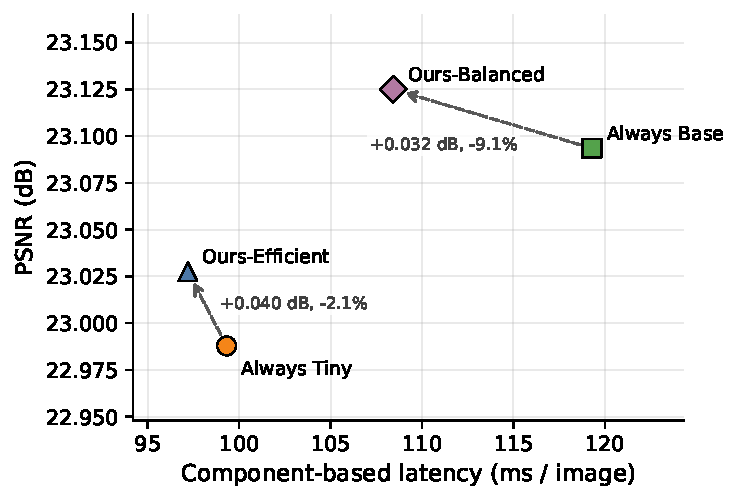
\includegraphics[width=\linewidth]{fig_psnr_latency_focus_v2.pdf}
        \caption{Quality-latency trade-off.}
        \label{fig:pareto}
    \end{subfigure}
    \hfill
    \begin{subfigure}{0.48\textwidth}
        \centering
        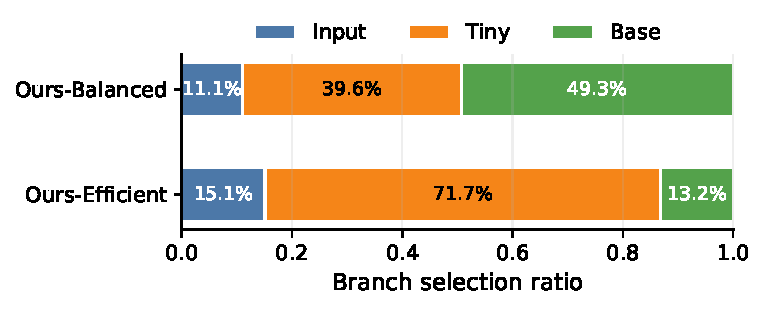
\includegraphics[width=\linewidth]{fig_action_ratio_horizontal_v2.pdf}
        \caption{Branch selection ratio.}
        \label{fig:action}
    \end{subfigure}
    \caption{
    FastGainRouter trades off restoration quality and computation.
    Always Input is omitted from (a) for readability and is reported in Table~\ref{tab:main}.
    }
    \label{fig:tradeoff-action}
\end{figure*}

\subsection{Qualitative Results}

Figure~\ref{fig:qualitative} shows qualitative examples of adaptive branch selection.
The examples are not intended to claim state-of-the-art restoration quality.
Instead, they illustrate four different routing behaviors: skipping restoration, using Tiny when it is sufficient, using Base when necessary, and selecting a lower-cost branch in the efficient setting.

\begin{figure*}[!t]
    \centering
    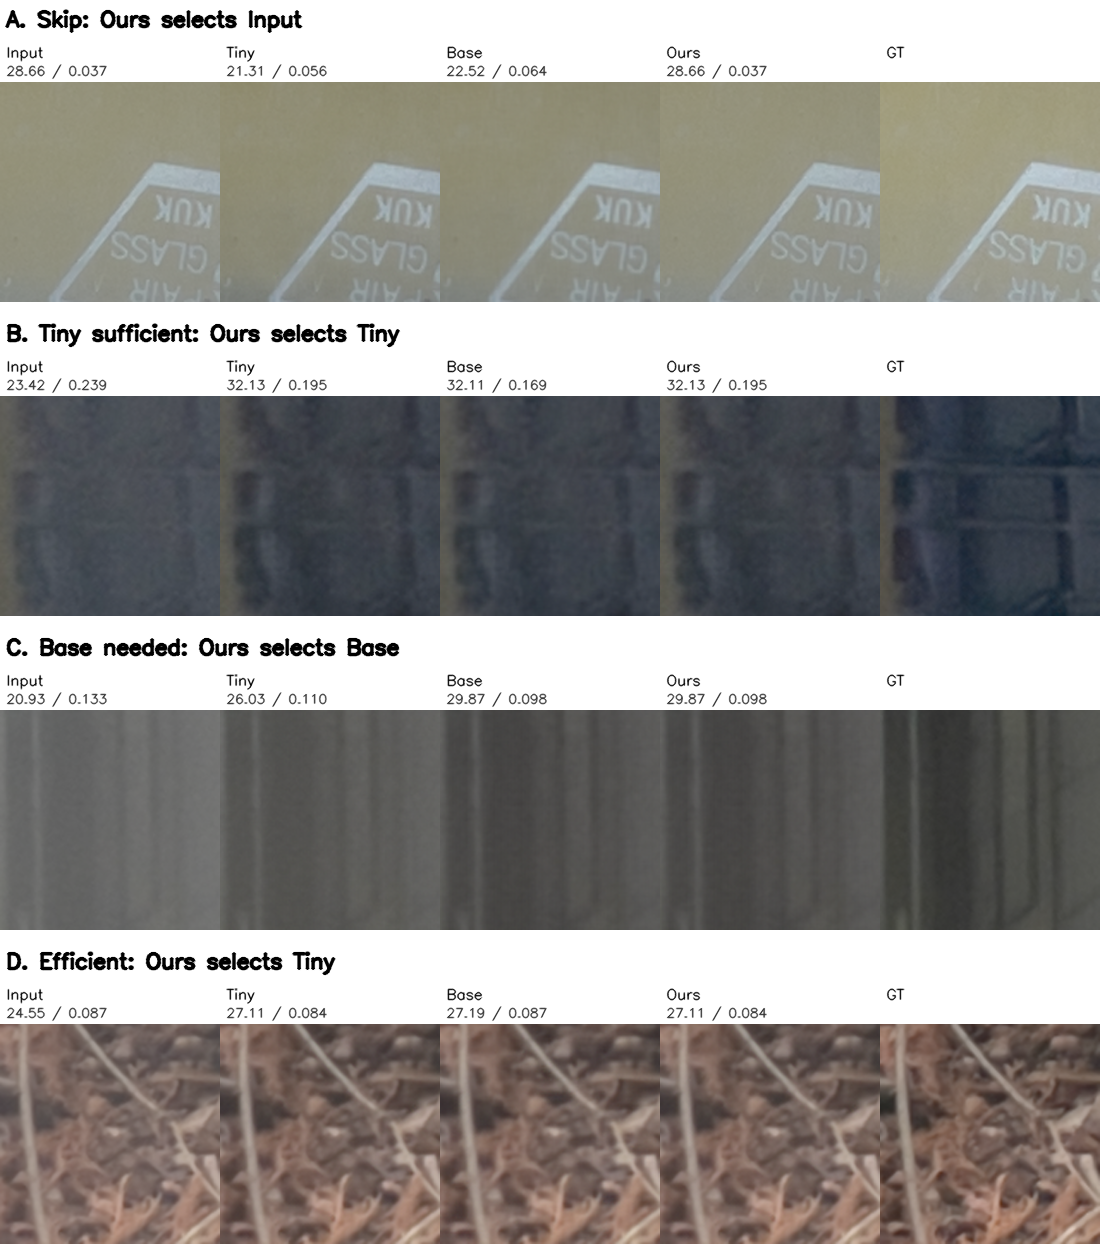
\includegraphics[width=0.92\textwidth,height=0.60\textheight,keepaspectratio]{qualitative_grid_v1.png}
    \caption{
    Qualitative examples of adaptive branch selection.
    Numbers indicate PSNR$\uparrow$ / LPIPS$\downarrow$.
    The rows show a skip case, a Tiny-sufficient case, a Base-needed case, and an efficient-routing case.
    }
    \label{fig:qualitative}
\end{figure*}

\FloatBarrier

% ------------------------------------------------------------
% 7. Discussion and Limitations
% ------------------------------------------------------------
\section{Discussion and Limitations}

\paragraph{Interpretation of small PSNR differences.}
Ours-Efficient loses only 0.066 dB PSNR compared with Always Base while reducing latency by 18.5\%.
Such a small average PSNR difference is modest in terms of pixel fidelity.
However, dirty-lens degradation may contain local artifacts such as water droplets, scratches, and scattering.
Therefore, PSNR should be interpreted together with LPIPS and qualitative examples.

\paragraph{Latency estimate.}
Our main latency is a component-based estimate, not a fully optimized deployment runtime.
It includes feature extraction, batch router prediction, and selected branch inference.
A naive single-image sklearn RandomForest implementation can introduce large overhead.
A deployment-oriented system should use optimized or neural router inference.

\paragraph{Router target generation.}
The router is trained using gain targets generated from train\_inner, which is also used to train Tiny and Base.
A stricter protocol could use cross-fitting or a separate router-training split so that gain targets are generated on restoration-unseen cases.
We leave this as future work.
The official validation set is held out and used only for final evaluation.

\paragraph{Restoration quality.}
This work does not aim to achieve state-of-the-art restoration quality.
Tiny and Base are intentionally small NAFNet variants used to study adaptive restoration budget selection.
Severe dirty-lens degradations may still require stronger restoration models.

% ------------------------------------------------------------
% 8. Conclusion
% ------------------------------------------------------------
\section{Conclusion}

We studied input-adaptive restoration for smartphone images with dirty lenses.
Building on the SIDL benchmark, we asked whether every dirty-lens image requires the same restoration budget.
We constructed Input, Tiny, and Base branches and proposed FastGainRouter, which predicts restoration gains from lightweight image statistics and selects a branch accordingly.

Our results show that Input, Tiny, and Base are each optimal for a substantial subset of validation samples.
FastGainRouter improves the quality-latency trade-off compared with fixed baselines.
In the balanced setting, it improves PSNR over Always Base while reducing latency.
In the efficient setting, it reduces latency substantially with only a small PSNR loss.
These results suggest that adaptive restoration budget selection is a promising direction for efficient dirty-lens image restoration.

\balance
\bibliographystyle{plain}
\bibliography{references}

\end{document}
